\documentclass{article}
\usepackage[letterpaper]{geometry}
\usepackage{amsmath} % for the equation* environment
\usepackage{tkz-euclide}
%\usetkzobj{all}

\title{C\'alculo de la tensi\'on de dos cuerdas en condici\'on de equilibrio que sostienen un cuerpo de $100 N$}
\date{Setiembre - 2024}
\author{por Oscar G. Pav\'on}


\begin{document}
  \pagenumbering{gobble}
  \maketitle
  \pagenumbering{arabic}



%problema
\begin{tikzpicture}[scale=1.7]

\tkzDefPoint(0,0){ZERO}


\tkzDefPoint(3,3){tB}
  \tkzDrawSegment[line width=1.0pt](ZERO,tB)

\tkzDefPoint(-3,3){tC}
  \tkzDrawSegment[line width=1.0pt](ZERO,tC)


  \tkzLabelAngle[pos=1](tC,tB,ZERO){$30 ^{\circ}$}
  \tkzLabelAngle[pos=-1](tB,tC,ZERO){$60 ^{\circ}$}

  \tkzDefPoint(3,0){tD}

  \tkzDefPoint(-3,0){tE}

\tkzDefPoint(0,-3){tF}
  \tkzDrawSegment[line width=1.0pt](ZERO,tF)

%\tkzDefPoint(0.1,0.1){A}
%\tkzDefPoint(-0.1,0.1){B}
%\tkzDefPoint(-0.1,-0.1){C}
%\tkzDefPoint(0.1,-0.1){D}


  \tkzDefPoint(0.6,-3.8){A}
  \tkzDefPoint(0.6,-3){B}
  \tkzDefPoint(-0.6,-3.8){D}
  \tkzDefPoint(-0.6,-3){C}
\tkzDrawPolygon(A,B,C,D)
  \tkzDefBarycentricPoint(A=1,B=1,C=1,D=1) \tkzGetPoint{P}
  \tkzLabelPoint[anchor=center](P){$P$}
  \tkzLabelSegment[right](A,B){$100 N$}

\end{tikzpicture}

Supongamos que tenemos dos cuerdas conectados entre si y hay una fuerza en el medio que va tirando de ellos. Esta fuerza es de $100 N$. Calcularemos la tensi\'on de las dos cuerdas
\newpage
Creamos un plano cartesiano:\newline
\begin{tikzpicture}[scale=.8]
\tkzDefPoint(0,0){ZERO}


\tkzDefPoint(3,3){tB}
\tkzDrawSegment(ZERO,tB)

\tkzDefPoint(-3,3){tC}
\tkzDrawSegment(ZERO,tC)


  \tkzLabelAngle[pos=1](tC,tB,ZERO){$30 ^{\circ}$}
  \tkzLabelAngle[pos=-1](tB,tC,ZERO){$60 ^{\circ}$}

  \tkzDefPoint(3,0){tD}

  \tkzDefPoint(-3,0){tE}

\tkzDefPoint(0,-3){tF}
\tkzDrawSegment(ZERO,tF)

  \tkzDefPoint(0.6,-3.8){A}
  \tkzDefPoint(0.6,-3){B}
  \tkzDefPoint(-0.6,-3.8){D}
  \tkzDefPoint(-0.6,-3){C}
\tkzDrawPolygon(A,B,C,D)
  \tkzDefBarycentricPoint(A=1,B=1,C=1,D=1) \tkzGetPoint{P}
  \tkzLabelPoint[anchor=center](P){$P$}
  \tkzLabelSegment[right](A,B){$100 N$}


\tkzDefPoint(0,0){A}
\tkzDefPoint(5,0){B}
\tkzDefPoint(0,5){C}
\tkzDefPoint(0,-5){D}
\tkzDefPoint(-5,0){E}


  \tkzDrawSegment[line width=1pt](A,B)
\tkzDrawSegment[line width=1pt](A,C)
\tkzDrawSegment[line width=1pt](A,D)
\tkzDrawSegment[line width=1pt](A,E)

\tkzLabelPoint(B){$x +$}
\tkzLabelPoint[right](C){$y +$}

\tkzLabelPoint[right](D){$ - y $}


\tkzLabelPoint(E){$ - x$}

\end{tikzpicture}


Unimos los puntos $A$ y $B$ para formar un tri\'angulo:\newline
\begin{tikzpicture}[scale=.8]
\tkzDefPoint(0,0){ZERO}


\tkzDefPoint(3,3){tB}
\tkzDrawSegment(ZERO,tB)

\tkzDefPoint(-3,3){tC}
\tkzDrawSegment(ZERO,tC)


  \tkzLabelAngle[pos=1](tC,tB,ZERO){$30 ^{\circ}$}
  \tkzLabelAngle[pos=-1](tB,tC,ZERO){$60 ^{\circ}$}

  \tkzDefPoint(3,0){tD}

  \tkzDefPoint(-3,0){tE}

\tkzDefPoint(0,-3){tF}
\tkzDrawSegment(ZERO,tF)

  \tkzDefPoint(0.6,-3.8){A}
  \tkzDefPoint(0.6,-3){B}
  \tkzDefPoint(-0.6,-3.8){D}
  \tkzDefPoint(-0.6,-3){C}
\tkzDrawPolygon(A,B,C,D)
  \tkzDefBarycentricPoint(A=1,B=1,C=1,D=1) \tkzGetPoint{P}
  \tkzLabelPoint[anchor=center](P){$P$}
  \tkzLabelSegment[right](A,B){$100 N$}


\tkzDefPoint(0,0){A}
\tkzDefPoint(5,0){B}
\tkzDefPoint(0,5){C}
\tkzDefPoint(0,-5){D}
\tkzDefPoint(-5,0){E}


  \tkzDrawSegment(A,B)
\tkzDrawSegment(A,C)
\tkzDrawSegment(A,D)
\tkzDrawSegment(A,E)

  \tkzDrawSegment[line width=1pt](tC,tB)
  \tkzLabelPoint[left](tC){$A$}
  \tkzLabelPoint[right](tB){$B$}
  \tkzDrawPoint(tC)
  \tkzDrawPoint(tB)

\tkzLabelPoint(B){$x +$}
\tkzLabelPoint[right](C){$y +$}

\tkzLabelPoint[right](D){$ - y $}


\tkzLabelPoint(E){$ - x$}

\end{tikzpicture}

Como el nuevo tri\'angulo esta divido en dos por el eje $y +$ obtenemos dos tri\'angulos rectangulos. Los tri\'angulos $A$ y $B$\newline

\begin{tikzpicture}[scale=.8]
\tkzDefPoint(0,0){ZERO}


\tkzDefPoint(3,3){tB}
  \tkzDrawSegment[line width=1.0pt](ZERO,tB)

\tkzDefPoint(-3,3){tC}
  \tkzDrawSegment[line width=1.0pt](ZERO,tC)

\tkzDefPoint(0,3){tF}
  \tkzDrawSegment[line width=1.0pt](ZERO,tF)
  
  \tkzDefBarycentricPoint(tB=1,tF=1,A=1) \tkzGetPoint{t1}

  \tkzLabelPoint[anchor=center](t1){$B$}
  
  \tkzDefBarycentricPoint(tC=1,tF=1,A=1) \tkzGetPoint{t2}

  \tkzLabelPoint[anchor=center](t2){$A$}

  \tkzDefPoint(3,0){tD}

  \tkzDefPoint(-3,0){tE}

\tkzDefPoint(0,-3){tF}
\tkzDrawSegment(ZERO,tF)

  \tkzDefPoint(0.6,-3.8){A}
  \tkzDefPoint(0.6,-3){B}
  \tkzDefPoint(-0.6,-3.8){D}
  \tkzDefPoint(-0.6,-3){C}
\tkzDrawPolygon(A,B,C,D)
  \tkzDefBarycentricPoint(A=1,B=1,C=1,D=1) \tkzGetPoint{P}
  \tkzLabelPoint[anchor=center](P){$P$}
  \tkzLabelSegment[right](A,B){$100 N$}


\tkzDefPoint(0,0){A}
\tkzDefPoint(5,0){B}
\tkzDefPoint(0,5){C}
\tkzDefPoint(0,-5){D}
\tkzDefPoint(-5,0){E}


  \tkzDrawSegment(A,B)
\tkzDrawSegment(A,C)
\tkzDrawSegment(A,D)
\tkzDrawSegment(A,E)

  \tkzDrawSegment[line width=1pt](tC,tB)

\tkzLabelPoint(B){$x +$}
\tkzLabelPoint[right](C){$y +$}

\tkzLabelPoint[right](D){$ - y $}


\tkzLabelPoint(E){$ - x$}

\end{tikzpicture}

Como son tri\'angulos rectangulos, osea que uno de sus \'angulos mide $90 ^{\circ}$. Podr\'iamos trazar l\'ineas del punto $A$ al eje $x$ y del punto $B$ al eje $x$. Obteniendo los tri\'angulos rectangulos $C$ y $D$.\newline
\begin{tikzpicture}[scale=.8]
\tkzDefPoint(0,0){ZERO}


\tkzDefPoint(3,3){tB}
\tkzDrawSegment(ZERO,tB)

\tkzDefPoint(-3,3){tC}
\tkzDrawSegment(ZERO,tC)



  \tkzDefPoint(3,0){tD}

  \tkzDefPoint(-3,0){tE}

\tkzDefPoint(0,-3){tF}
\tkzDrawSegment(ZERO,tF)

  \tkzDefPoint(0.6,-3.8){A}
  \tkzDefPoint(0.6,-3){B}
  \tkzDefPoint(-0.6,-3.8){D}
  \tkzDefPoint(-0.6,-3){C}
\tkzDrawPolygon(A,B,C,D)
  \tkzDefBarycentricPoint(A=1,B=1,C=1,D=1) \tkzGetPoint{P}
  \tkzLabelPoint[anchor=center](P){$P$}
  \tkzLabelSegment[right](A,B){$100 N$}


\tkzDefPoint(0,0){A}
\tkzDefPoint(5,0){B}
\tkzDefPoint(0,5){C}
\tkzDefPoint(0,-5){D}
\tkzDefPoint(-5,0){E}


  \tkzDrawSegment(A,B)
\tkzDrawSegment(A,C)
\tkzDrawSegment(A,D)
\tkzDrawSegment(A,E)

  \tkzDrawSegment(tC,tB)
  \tkzLabelPoint[left](tC){$A$}
  \tkzLabelPoint[right](tB){$B$}
  \tkzDrawPoint(tC)
  \tkzDrawPoint(tB)

\tkzDefPoint(3,0){tF}
  \tkzDrawSegment[line width=1.0pt](tB,tF)
  
  \tkzDefBarycentricPoint(tB=1,A=1,tF=1) \tkzGetPoint{t1}

  \tkzLabelPoint[anchor=center](t1){$C$}

  \tkzDefPoint(-3,0){tF}
  \tkzDrawSegment[line width=1.0pt](tC,tF)

  
  \tkzDefBarycentricPoint(tC=1,A=1,tF=1) \tkzGetPoint{t2}

  \tkzLabelPoint[anchor=center](t2){$D$}

\tkzLabelPoint(B){$x +$}
\tkzLabelPoint[right](C){$y +$}

\tkzLabelPoint[right](D){$ - y $}


\tkzLabelPoint(E){$ - x$}

\end{tikzpicture}

Los \'angulos de los tri\'angulos rectangulos $C$ y $D$ son los mismos que los tri\'angulos $A$ y $B$:\newline

\begin{tikzpicture}[scale=.8]
\tkzDefPoint(0,0){ZERO}


\tkzDefPoint(3,3){tB}
\tkzDrawSegment(ZERO,tB)

\tkzDefPoint(-3,3){tC}
\tkzDrawSegment(ZERO,tC)



  \tkzDefPoint(3,0){tD}

  \tkzDefPoint(-3,0){tE}

\tkzDefPoint(0,-3){tF}
\tkzDrawSegment(ZERO,tF)

  \tkzDefPoint(0.6,-3.8){A}
  \tkzDefPoint(0.6,-3){B}
  \tkzDefPoint(-0.6,-3.8){D}
  \tkzDefPoint(-0.6,-3){C}
\tkzDrawPolygon(A,B,C,D)
  \tkzDefBarycentricPoint(A=1,B=1,C=1,D=1) \tkzGetPoint{P}
  \tkzLabelPoint[anchor=center](P){$P$}
  \tkzLabelSegment[right](A,B){$100 N$}


\tkzDefPoint(0,0){A}
\tkzDefPoint(5,0){B}
\tkzDefPoint(0,5){C}
\tkzDefPoint(0,-5){D}
\tkzDefPoint(-5,0){E}


  \tkzDrawSegment(A,B)
\tkzDrawSegment(A,C)
\tkzDrawSegment(A,D)
\tkzDrawSegment(A,E)

  \tkzDrawSegment(tC,tB)

\tkzDefPoint(3,0){tF}
  \tkzDrawSegment(tB,tF)
  
  \tkzLabelAngle[pos=1](tF,ZERO,tB){$30 ^{\circ}$}
  \tkzMarkAngle[size=1.4cm](tF,ZERO,tB)

\tkzDefPoint(0,3){tF}
  \tkzLabelAngle[pos=1](ZERO,tC,tF){$60 ^{\circ}$}
  \tkzMarkAngle[size=1.4cm](ZERO,tC,tF)
  
  \tkzDefBarycentricPoint(tB=1,A=1,tF=1) \tkzGetPoint{t1}


  \tkzDefPoint(-3,0){tF}
  \tkzDrawSegment(tC,tF)

  \tkzLabelAngle[pos=1](tC,ZERO,tF){$60 ^{\circ}$}
  \tkzMarkAngle[size=1.4cm](tC,ZERO,tF)
  
  \tkzDefBarycentricPoint(tC=1,A=1,tF=1) \tkzGetPoint{t2}

  \tkzLabelAngle[pos=1](tC,tB,ZERO){$30 ^{\circ}$}
  \tkzMarkAngle[size=1.4cm](tC,tB,ZERO)

\tkzLabelPoint(B){$x +$}
\tkzLabelPoint[right](C){$y +$}

\tkzLabelPoint[right](D){$ - y $}


\tkzLabelPoint(E){$ - x$}

\end{tikzpicture}

Comenzaremos con el triaunglo $C$.\newline

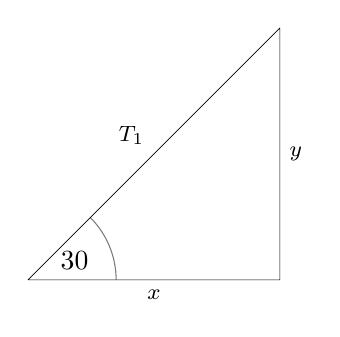
\begin{tikzpicture}[scale=.8]
%\tkzInit[xmax=5,ymax=3] %\tkzClip[space=.5]

\tkzDefPoint(0,0){A}
\tkzDefPoint(4,0){B}
\tkzDefPoint(4,4){C}


\tkzDrawPolygon(A,B,C)
\tkzLabelSegment[auto,font=\footnotesize](A,C){$T_1$}
\tkzLabelSegment[below,font=\footnotesize](A,B){$x$}
\tkzLabelSegment[right,font=\footnotesize](B,C){$y$}
\tkzMarkAngle[fill= blue!40,size=1.4cm,opacity=.5](B,A,C)
\tkzLabelAngle[pos=0.8](B,A,C){$30$}

\end{tikzpicture}
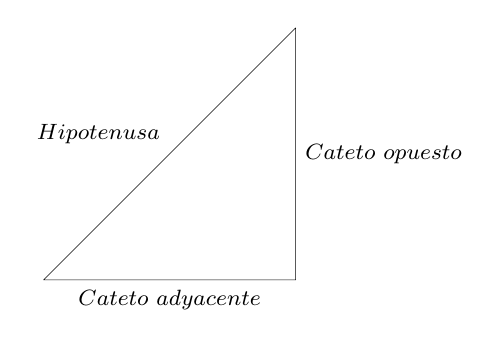
\begin{tikzpicture}[scale=.8]
%\tkzInit[xmax=5,ymax=3] %\tkzClip[space=.5]

\tkzDefPoint(0,0){A}
\tkzDefPoint(4,0){B}
\tkzDefPoint(4,4){C}


\tkzDrawPolygon(A,B,C)
\tkzLabelSegment[auto,font=\footnotesize](A,C){$Hipotenusa$}
\tkzLabelSegment[below,font=\footnotesize](A,B){$Cateto$ $adyacente$}
\tkzLabelSegment[right,font=\footnotesize](B,C){$Cateto$ $opuesto$}

\end{tikzpicture}

Debemos hallar el valor de $x$ y el valor de $y$ para por obtener el valor de la tensi\'on $T_1$. Para lograr esto utilizaremos el Teorema de Pit\'agoras.

Para obtener $x$ necesitamos el valor de $\cos \alpha$ y para $y$ el valor de $\sin \alpha$. Como necesitamos $x$ e $y$ de la $T_1$ y la $T_2$ utilizaremos:\newline $T_1x$ , $T_1y$ y $T_2x$ , $T_2y$.\newline


El Teorema de Pit\'agoras dice que:\newline

\qquad $\cos \alpha = \dfrac{\text{cateto adyacente}}{\text{hipotenusa}}$\qquad $\sin \alpha = \dfrac{\text{cateto opuesto}}{\text{hipotenusa}}$\newline\newline


\begin{math}
  \qquad \cos 30 = \dfrac{T_1x}{T_1}
  \qquad \sin 30 = \dfrac{T_1y}{T_1}
\end{math}

La regla fundamental de despeje, que resume las propiedades y leyes matemáticas que la sustentan, en términos sencillos dice:\newline 
Toda cantidad que se pasa de un lado a otro de la igualdad, debe pasar realizando la operación contraria.

Para hallar $T_1x$ se pasa $T_1$ al otro lado de la igualdad:\newline

$\cos 30 = \dfrac{T_1x}{T_1}$

$T_1 \cos 30 = T_1x$ por tanto:

$T_1x = T_1 \cos 30$\qquad($1$)\newline
Y repetimos para hallar $T_1y$

$\sin 30 = \dfrac{T_1y}{T_1}$

$T_1 \cos 60 = T_1y$

$T_1y = T_1 \cos 60$\qquad (2)\newline

Hallaremos $T_2$ con el tri\'angulo $D$

\begin{tikzpicture}[scale=.8]
\tkzDefPoint(0,0){ZERO}



\tkzDefPoint(-3,3){tC}
  \tkzDrawSegment[line width=1.0pt](ZERO,tC)
  \tkzLabelSegment[right](ZERO,tC){$T_2$}



  \tkzDefPoint(3,0){tD}

  \tkzDefPoint(-3,0){tE}

\tkzDefPoint(0,-3){tF}
\tkzDrawSegment(ZERO,tF)



\tkzDefPoint(0,0){A}
\tkzDefPoint(5,0){B}
\tkzDefPoint(0,5){C}
\tkzDefPoint(0,-5){D}
\tkzDefPoint(-5,0){E}


  \tkzDrawSegment(A,B)
\tkzDrawSegment(A,C)
\tkzDrawSegment(A,D)
\tkzDrawSegment(A,E)



  \tkzDefPoint(-3,0){tF}
  \tkzDrawSegment[line width=1.0pt](tC,tF)
  
  \tkzDrawSegment[line width=1.0pt](ZERO,tF)

  \tkzLabelSegment[left](tC,tF){$y$}
  \tkzLabelSegment[auto](ZERO,tF){$-x$}

  \tkzLabelAngle[pos=1](tC,ZERO,tF){$60 ^{\circ}$}
  \tkzMarkAngle[size=1.4cm](tC,ZERO,tF)
  
  \tkzDefBarycentricPoint(tC=1,A=1,tF=1) \tkzGetPoint{t2}


\tkzLabelPoint(B){$x +$}
\tkzLabelPoint[right](C){$y +$}

\tkzLabelPoint[right](D){$ - y $}


\tkzLabelPoint(E){$ - x$}

\end{tikzpicture}
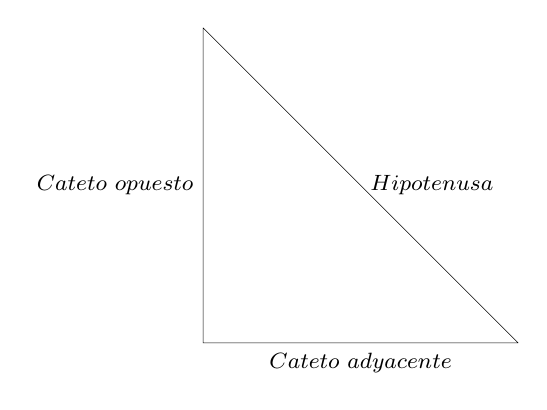
\begin{tikzpicture}[scale=1]
%\tkzInit[xmax=5,ymax=3] %\tkzClip[space=.5]

\tkzDefPoint(0,0){A}
\tkzDefPoint(-4,0){B}
\tkzDefPoint(-4,4){C}


\tkzDrawPolygon(A,B,C)
  \tkzLabelSegment[right,font=\footnotesize](A,C){$Hipotenusa$}
\tkzLabelSegment[below,font=\footnotesize](A,B){$Cateto$ $adyacente$}
\tkzLabelSegment[left,font=\footnotesize](B,C){$Cateto$ $opuesto$}

\end{tikzpicture}

El Teorema de Pit\'agoras dice que:\newline

\qquad $\cos \alpha = \dfrac{\text{cateto adyacente}}{\text{hipotenusa}}$\qquad $\sin \alpha = \dfrac{\text{cateto opuesto}}{\text{hipotenusa}}$\newline\newline


\begin{math}
  \qquad \cos 60 = \dfrac{T_2x}{T_2}
  \qquad \sin 60 = \dfrac{T_2y}{T_2}
\end{math}\newline
Para hallar $T_2x$ se pasa $T_2$ al otro lado de la igualad y queda:\newline

$\cos 60 = \dfrac{T_2x}{T_2}$

$T_2 \cos 60 = T_2x$ por tanto:

$T_2x = T_2 \cos 60$\qquad (3)\newline


$\sin 60 = \dfrac{T_2y}{T_2}$

$T_2 \sin 60 = T_2y$ por tanto:

$T_2y = T_2 \sin 60$\qquad (4)\newline


C\'alculo de la condici\'on de equilibrio\newline

\qquad $\Sigma F_x = 0$\newline

El s\'imbolo $\Sigma$ es una letra griega en may\'uscula que significa la suma de todos los miembros y la $F$ es la fuerza\newline
La suma de las fuerzas en el eje $x$ es igual a cero\newline
Entonces tendr\'iamos:\newline

\qquad $T_1x + T_2x = 0$\newline

Reemplazamos utilizando las f\'ormulas obtenidas (1) (2):\newline

\qquad $T_1 \cos 30 + (- T_2 cos 60) = 0$\newline
Menos por m\'as es igual a menos, entonces tendr\'iarmos:\newline

\qquad $T_1 \cos 30 - T_2 \cos 60 = 0$\newline

Calculamos:\newline
$\cos 30 = 0.866$\newline
$\cos 60 = 0.5$\newline

\qquad $T_1 0.866 - T_2 0.5 = 0$\newline

Pasamos el valor de $T_2x$ = $-T_2 0.5$ al otro miembro\newline

\qquad $T_1 0.866 = T_2 0.5$\newline

Y para calcular $T_1$ pasamos $0.866$ al otro miembro. Y como esta multiplicando pasa a estar dividiendo\newline

\qquad $T_1 = \dfrac{T_2 0.5}{0.866}$\newline

Resolvemos:\newline

\qquad$\frac{0.5}{0.866} = 0.577$\newline

\qquad $T_1 = T_2 0.577$ \qquad (5) \newline

Hallar $T_2$:\newline

\qquad $\Sigma F_y = 0$\newline

La suma de las fuerzas en el eje $y$ es igual a cero\newline

En el eje $y$ hay una fuerza que est\'a en lado negativo, es la $P$ y su valor es de $100N$

$T_1y + T_2y + P = 0$\newline\newline
Calculamos $sin 60$ y $sen 60$\newline

$T_1 \sin 30 + T_2 \sin 60 + (-100 N) = 0$\qquad (5)\newline

$T_1 0.5 + T_2 0.866 -100 N = 0$\newline\newline
Usamos el valor de (5) y remplazamos $T_1$\newline

$T_2 0.577 \times 0.5 + T_2 0.866 - 100 N = 0$\newline\newline
Resolvemos $0.577 \times 0.5$\newline

$T_2 0.288 + T_2 0.866 - 100 N = 0$\newline\newline
Pasamos $100 N$ al otro miembro\newline

$T_2 0.288 + T_2 0.866 = 100 N$\newline\newline
Usamos el factor com\'un\newline

$T_2 ( 0.288 + 0.866 ) = 100 N$\newline\newline
Pasamos $1.154$ al otro miembro de la igualdad\newline

$T_2 1.154 = 100 N$\newline

$T_2 = \dfrac{100 N}{1.154}$\newline

$T_2 = 86.62 N$\qquad (R)\newline\newline
$T_1 = 86.62 N \times 0.577$\newline

$T_1 = 50 N$\qquad (R)\newline

Como resultado tenemos que la tensi\'on de la cuerda $1$ es $50 N$ y la tensi\'on de la cuerda $2$ es $86.63 N$
\end{document}
